\documentclass[a4paper,12pt]{jarticle}
\input ./chap01_preamble.tex
\graphicspath{%
  {../text01-img/}%
}
% !TEX root = ./chap01_03.tex
\begin{document}
\section[ラズベリーパイになれよう(2)]{ラズベリーパイになれよう(2)}
\subsection{写真をさつえいしよう}
\refstepcounter{Exercise}
\subsection{\theExercise ウェブカメラで写真をさつえいしよう}
\addtocounter{Exercise}{-1}\refstepcounter{Exercise}\label{E:webcam}
ウェブカメラを使用して\ruby{画像}{がぞう}をさつえいをします。

まずは、ラズベリーパイにウェブカメラを\ruby{接続}{せつぞく}しましょう。キーボードやマウスと同じように、ウェブカメラのUSBのたんしをラズベリーパイのUSBたんしへ差し\ruby{込}{こ}みます。



\begin{figure}[ht]
  \centering
  \begin{minipage}{8.528cm}
    {\upshape
      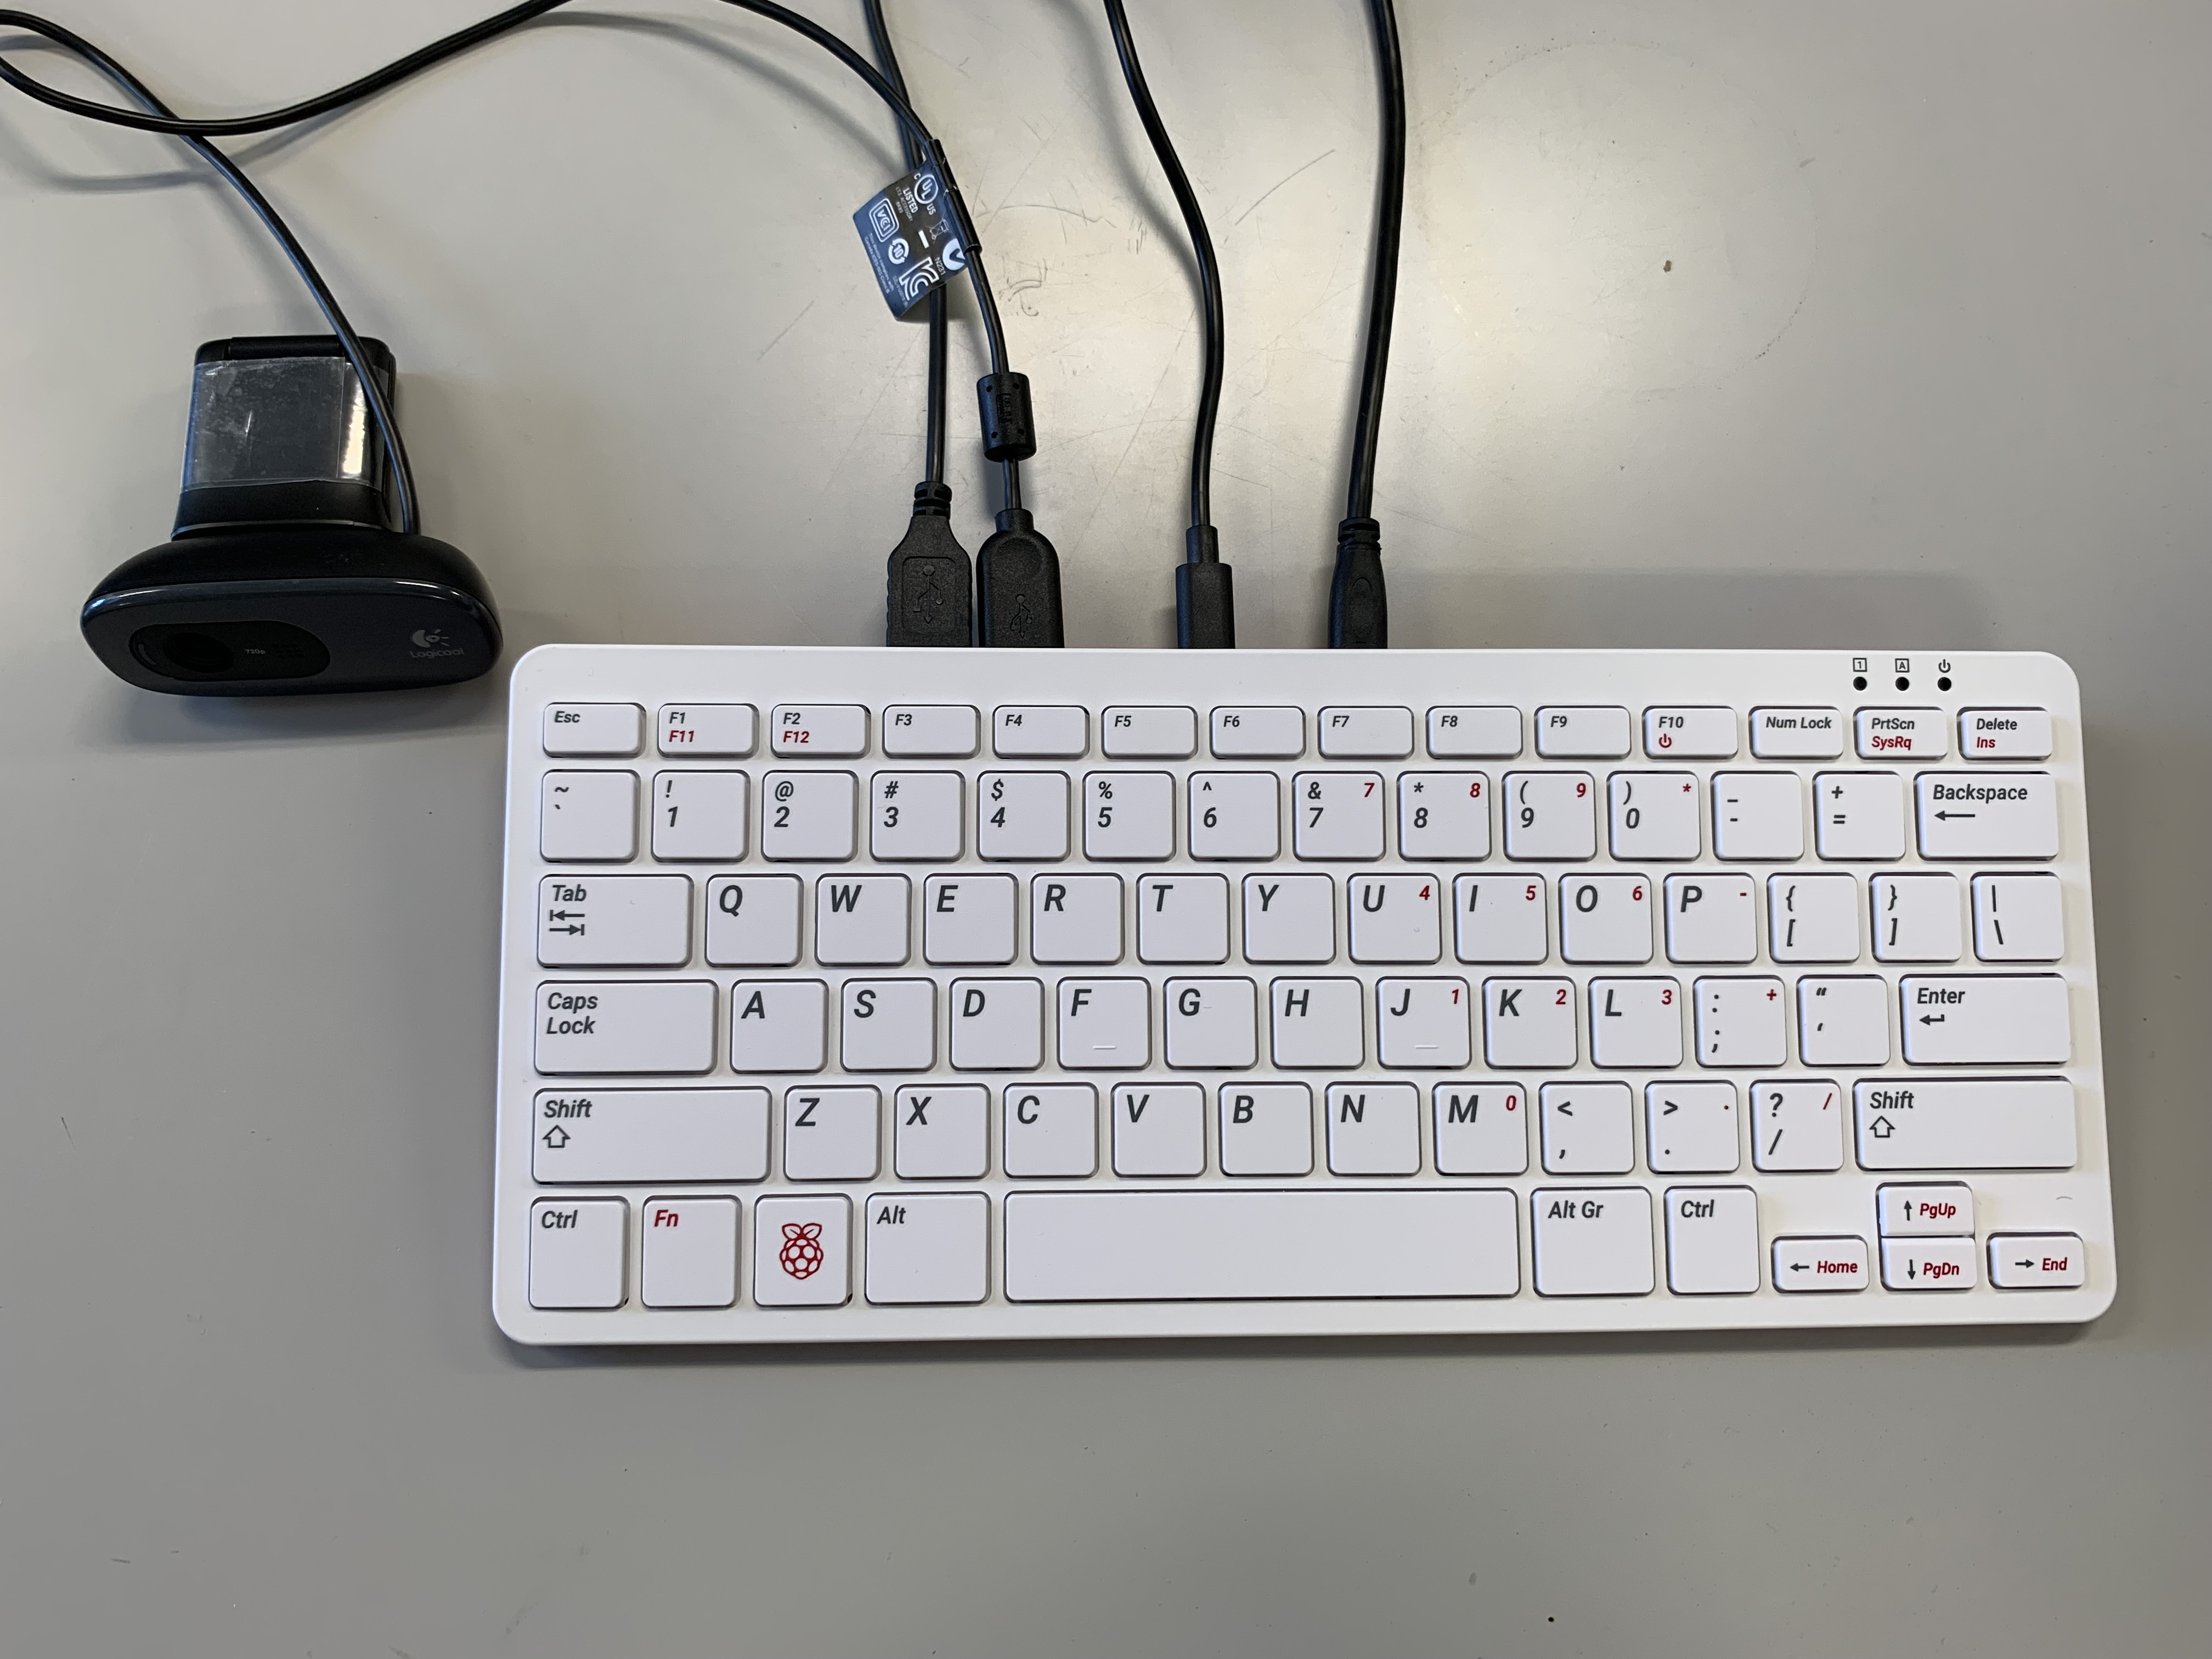
\includegraphics[width=7.904cm,height=5.928cm]{textbook-img112-2023.jpg}
      \newline
      Figure \stepcounter{Figure}{\theFigure}: Webカメラの接続}
  \end{minipage}
\end{figure}
ウェブカメラを接続したら、ラズベリーパイからウェブカメラの画像を取得してみましょう。左上のラズベリーのアイコンをクリックします。そこから、サウンドとメディアを\ruby{選択}{せんたく}しVLCメディアプレーヤーをクリックします。

\begin{figure}[hb]
  \centering
  \begin{minipage}{10.917cm}
    {\upshape
      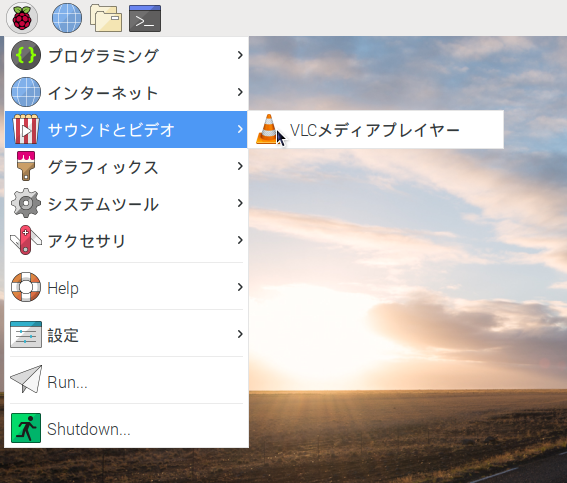
\includegraphics[width=10.232cm,height=8.715cm]{textbook-img113.png}
      \newline
      Figure \stepcounter{Figure}{\theFigure}: メニューからVLC起動}
  \end{minipage}
\end{figure}
\clearpage
\begin{figure}[ht]
  Figure~\ref{seq:refFigure20}のようにVLCメディアプレーヤーが起動します。



  \centering
  \begin{minipage}{9.684cm}
    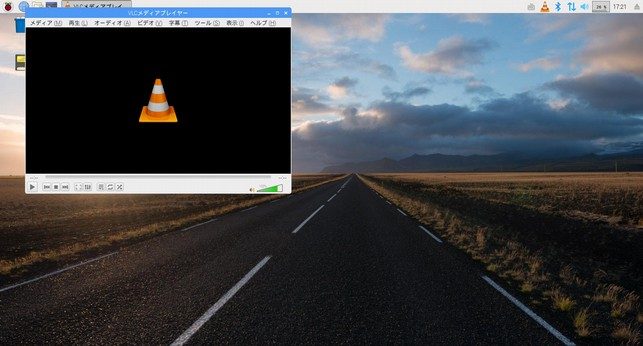
\includegraphics[width=9.948cm,height=5.364cm]{textbook-img114.jpg}


    Figure {\refstepcounter{Figure}\theFigure\label{seq:refFigure20}}: VLC起動画面
  \end{minipage}
  \flushleft
  VLCが起動したら\ruby{確認}{かくにん}メッセージが出てきます。

  \textbf{\textcolor[rgb]{1.0,0.2,0.2}{赤わくで囲われているチェックボックスにチェックマーク(\CheckedBox)}}がついていないことを確認して続けるをクリックしてください。



  \centering
  \begin{minipage}{7.186cm}
    {\upshape
      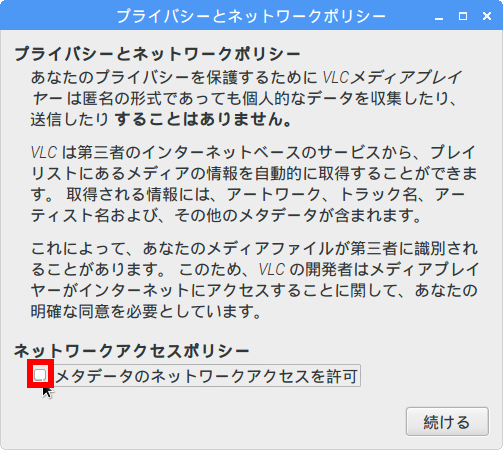
\includegraphics[width=7.2cm,height=7.0cm]{textbook-img115.png}
      \newline
      Figure \stepcounter{Figure}{\theFigure}: 確認メッセージ}
  \end{minipage}

  \flushleft
  カメラを開きます。Figure~\ref{seq:refFigure22}のように\textbf{メディア}をクリックして\textbf{キャプチャーデバイスを開く}をクリックします。


  \centering
  \begin{minipage}{8.096cm}
    {\upshape
      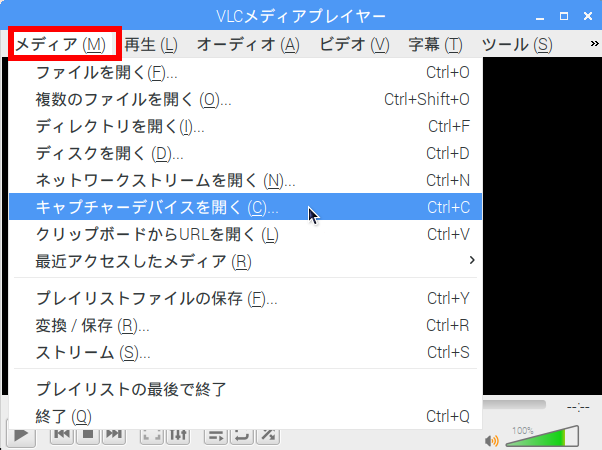
\includegraphics[width=8.0cm,height=7.0cm]{textbook-img116.png}
      \newline
      Figure {\refstepcounter{Figure}\theFigure\label{seq:refFigure22}}:
      キャプチャデバイスをひらく}
  \end{minipage}
\end{figure}
\clearpage

\begin{figure}[ht]
  Figure~\ref{seq:refFigure23}のような画面がでてきます。
  赤線で囲われている\textbf{キャプチャーモード}を
  \textbf{Video camera}にして
  青線で囲われている\textbf{\ruby{再生}{さいせい}}をクリックします。


  \centering
  \begin{minipage}{9.119cm}
    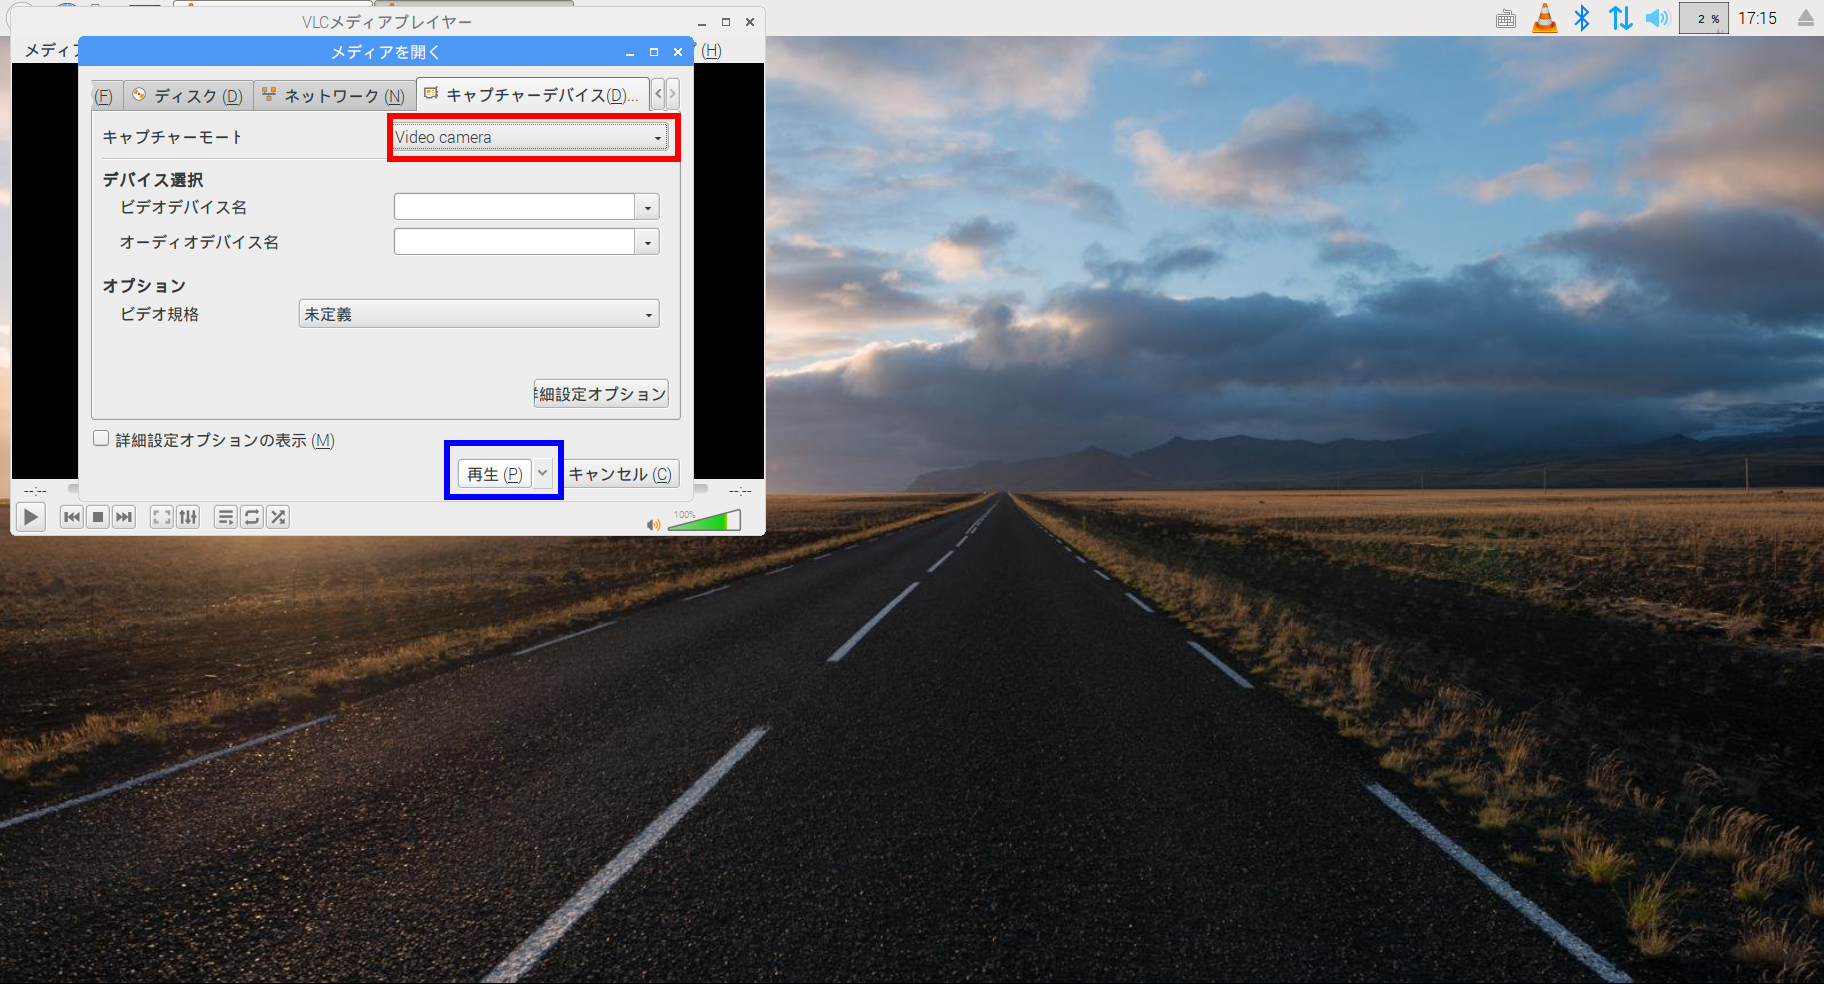
\includegraphics[width=8.915cm,height=6.426cm]{textbook-img117.png}
    Figure {\refstepcounter{Figure}\theFigure\label{seq:refFigure23}}:
    キャプチャーデバイスを開く画面
  \end{minipage}

  \flushleft
  しばらくすると、カメラの画像が見えるようになります。

  \centering
  \begin{minipage}{9.125cm}
    {\upshape
      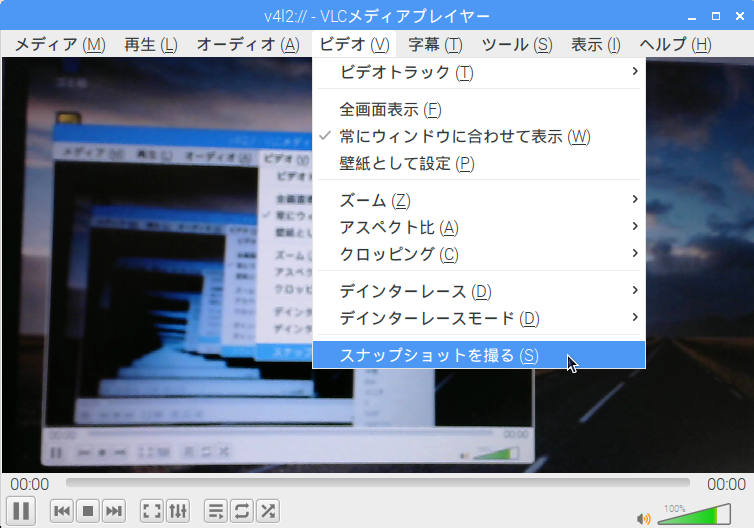
\includegraphics[width=8.966cm,height=6.274cm]{textbook-img118.png}
      \newline
      Figure \stepcounter{Figure}{\theFigure}: スナップショット\ruby{撮影}{さつえい}}
  \end{minipage}
  \flushleft

  次に、カメラでさつえいしてみましょう。ビデオをクリックしてスナップショットを撮るをクリックします。


  \centering
  \begin{minipage}{9.156cm}
    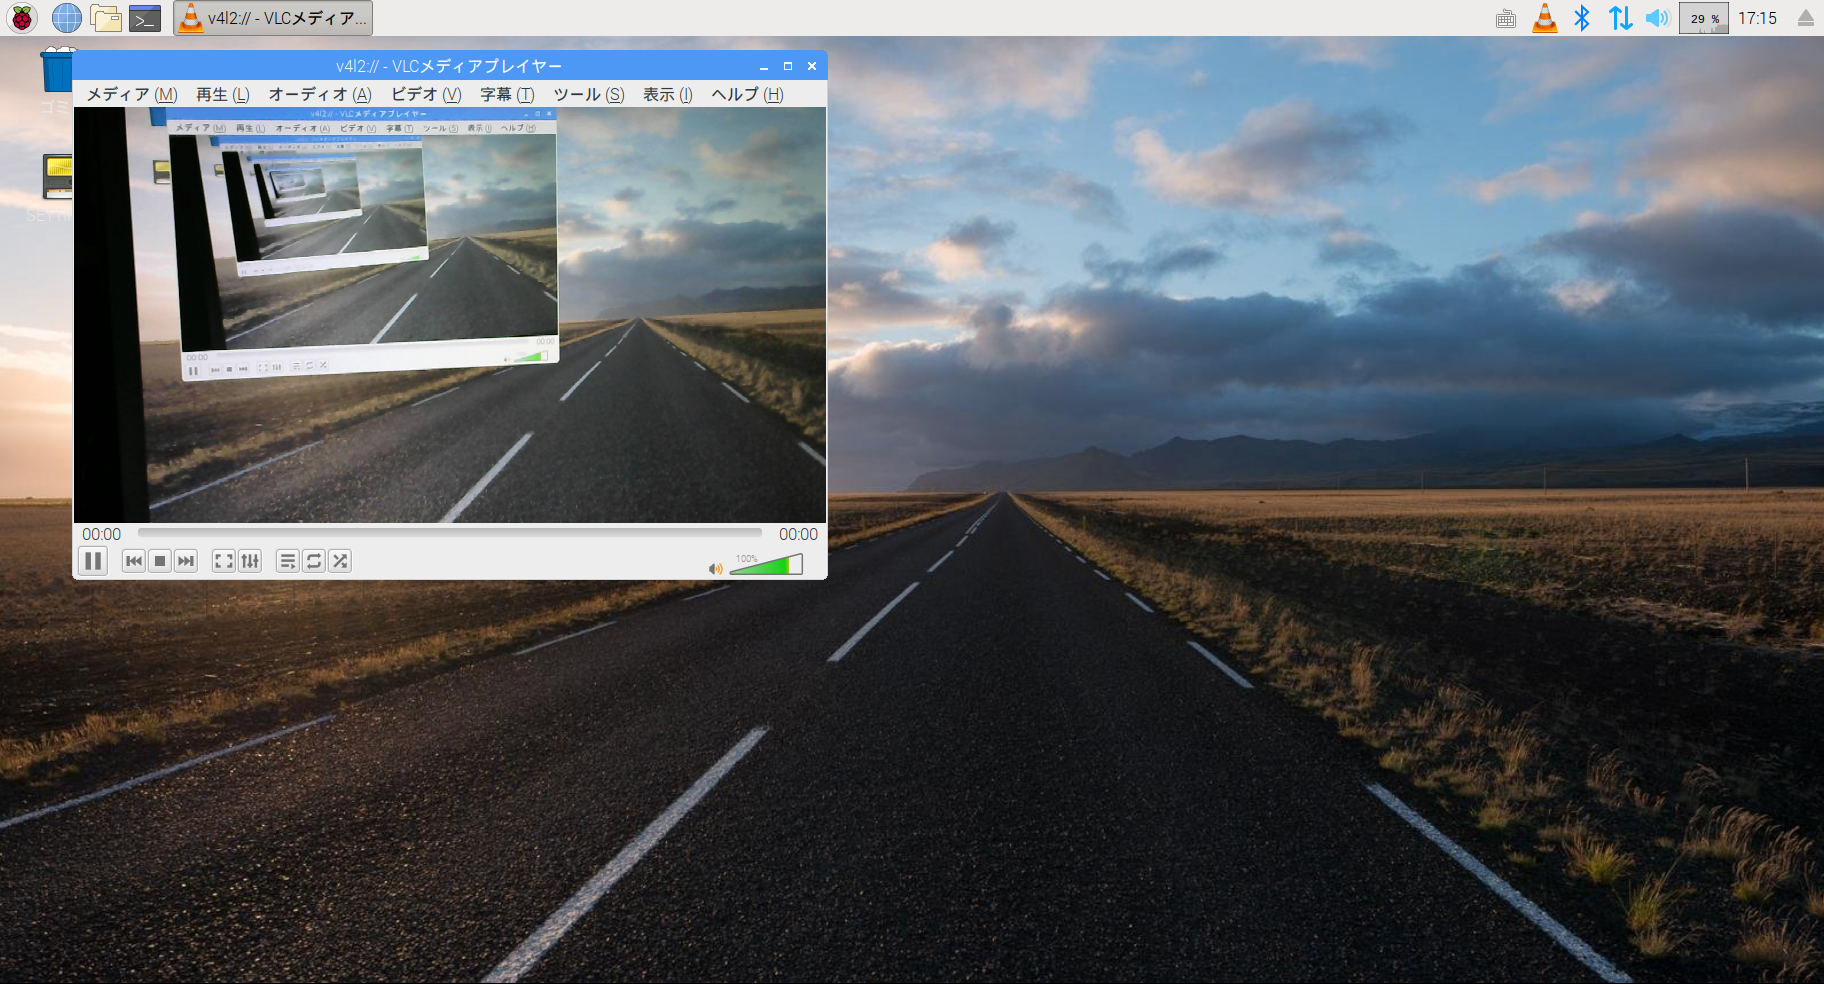
\includegraphics[width=9.042cm,height=6.426cm]{textbook-img119.png}
    {\upshape
      Figure \stepcounter{Figure}{\theFigure}: カメラ入力}
  \end{minipage}
\end{figure}
\clearpage
\begin{figure}
  黒線の四角に囲われたように\ruby{保存}{ほぞん}場所が表示され、そこへ画像が保存されます。

  \centering
  \begin{minipage}{9.206cm}
    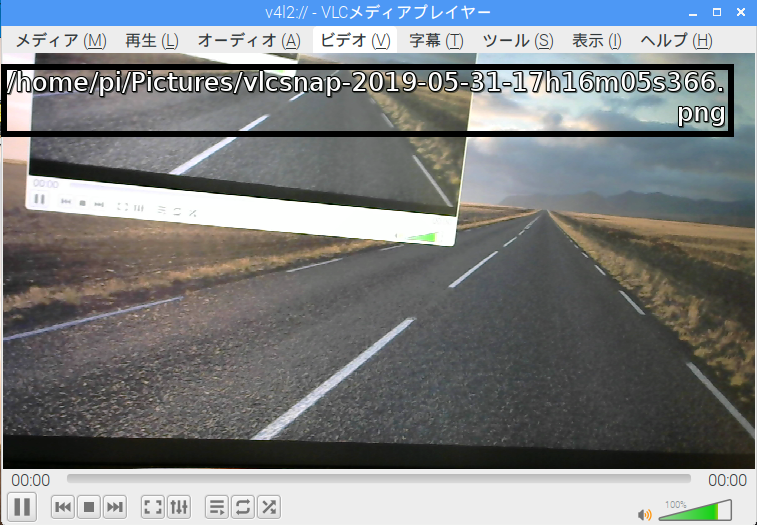
\includegraphics[width=9.017cm,height=6.248cm]{textbook-img120.png}
    Figure \stepcounter{Figure}{\theFigure}: スナップショット保存
  \end{minipage}



  \bigskip
  \flushleft

  初期\ruby{状態}{じょうたい}ではPicturesの下に保存されます。確認してみましょう。



  \centering
  \begin{minipage}{9.345cm}
    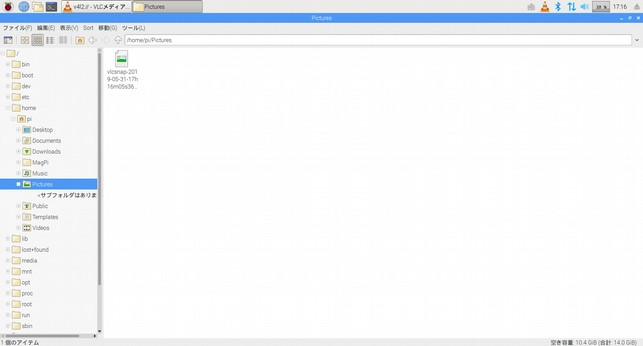
\includegraphics[width=9.22cm,height=5.306cm]{textbook-img121.jpg}

    Figure \stepcounter{Figure}{\theFigure}: 画像撮影場所
  \end{minipage}


  \bigskip

  \flushleft
  とった画像を確認してみましょう。Figure~\ref{seq:refFigure28}の赤わくで囲ってあるものがとった写真です。ダブルクリックをすると、画像を開いて見ることができます。



  \centering
  \begin{minipage}{9.162cm}
    {\upshape
      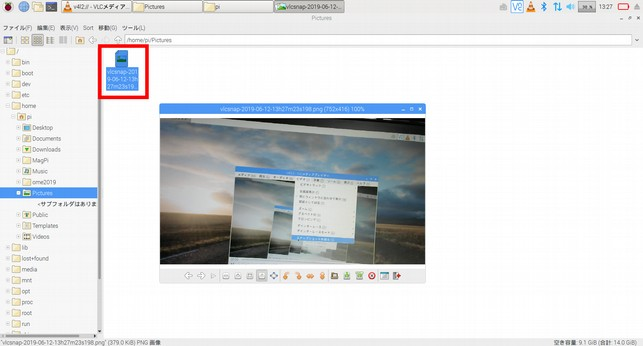
\includegraphics[width=9.125cm,height=5.182cm]{textbook-img122.jpg}
      \newline
      Figure {\refstepcounter{Figure}\theFigure\label{seq:refFigure28}}:
      とった画像を開く}
  \end{minipage}
\end{figure}

\bigskip

\clearpage

\begin{figure}[ht]
  \refstepcounter{Exercise}
  \subsection{\theExercise 画像に絵をかこう}

  \bigskip

  “GIMP”ソフトを立ち上げて、色付きの筆で自分の顔写真に絵をかこう

  画像を開いて、色を選択、お絵かきツールの筆を選んで書くよ

  \textbf{考え方}



  \begin{minipage}{\textwidth}
    \centering
    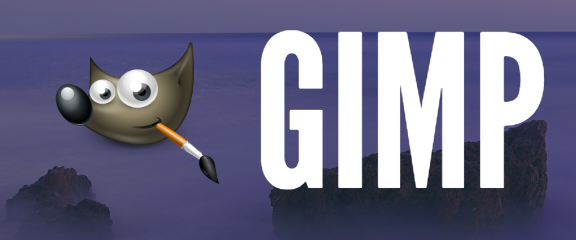
\includegraphics[width=6.112cm,height=2.284cm]{textbook-img123.png}
    \begin{minipage}[b]{8.617cm}

      本格的な画像編集、加工ソフトの

      GIMPを使って自分の顔写真などの

      画像を\ruby{編集}{へんしゅう}してみよう
    \end{minipage}


  \end{minipage}
  \bigskip




  \begin{minipage}{\textwidth}
    \centering
    \begin{minipage}{5.852cm}
      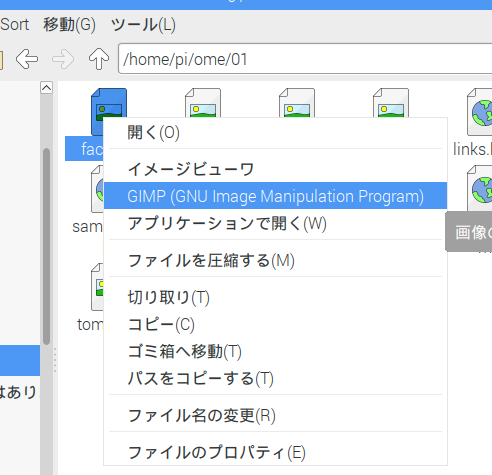
\includegraphics[width=5.359cm,height=5.258cm]{textbook-img124.png}\\
      1 編集したい画像ファイルを

      右クリックしGIMPをクリック
    \end{minipage}
    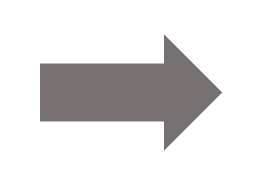
\includegraphics[width=1.489cm,height=1.365cm]{textbook-img128.png}
    \begin{minipage}{7.975cm}
      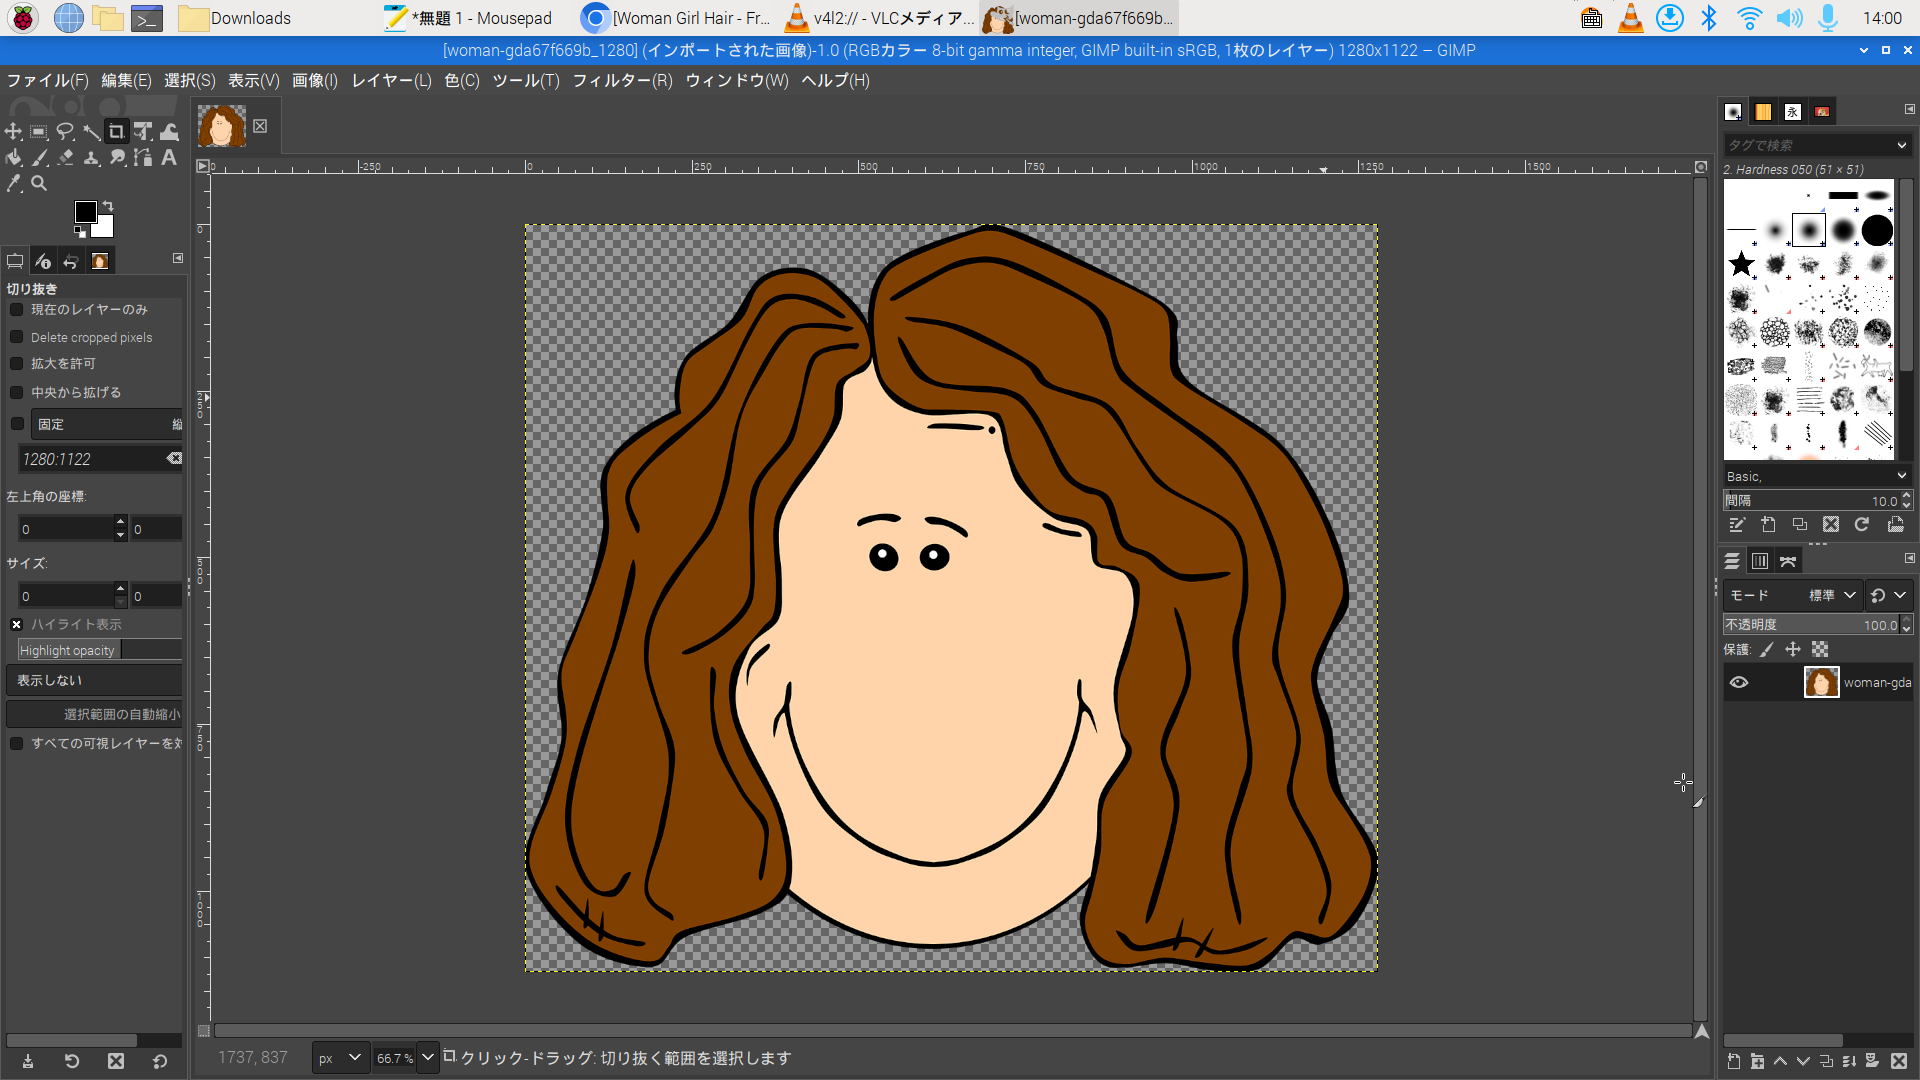
\includegraphics[width=7.65cm,height=4.426cm]{textbook-img125.png}\\
      2 画像編集モードになるよ
    \end{minipage}


  \end{minipage}
  \bigskip




  \begin{minipage}{\textwidth}
    \begin{minipage}{5.984cm}
      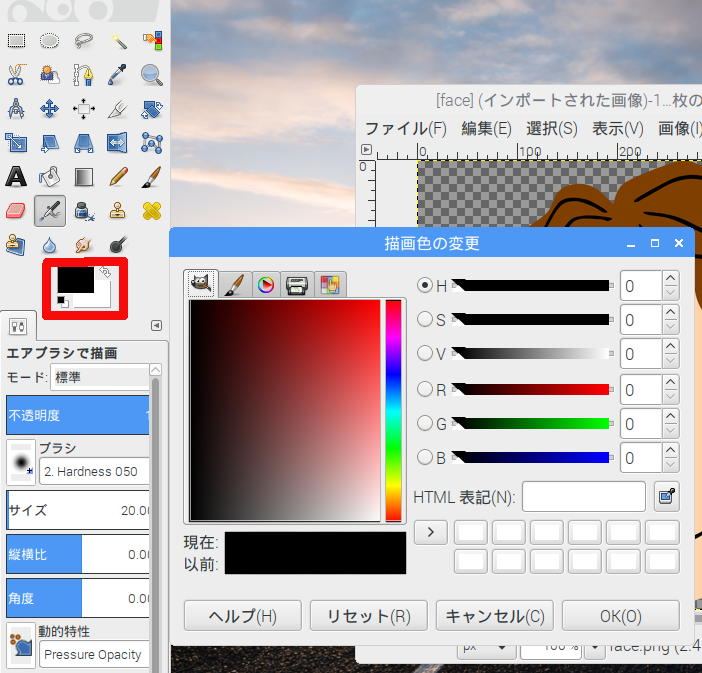
\includegraphics[width=5.971cm,height=5.738cm]{textbook-img129.png}\\
      3 赤い丸で囲まれている

      部分をクリック


      \bigskip
    \end{minipage}
    \hfill
    \begin{minipage}{8.984cm}
      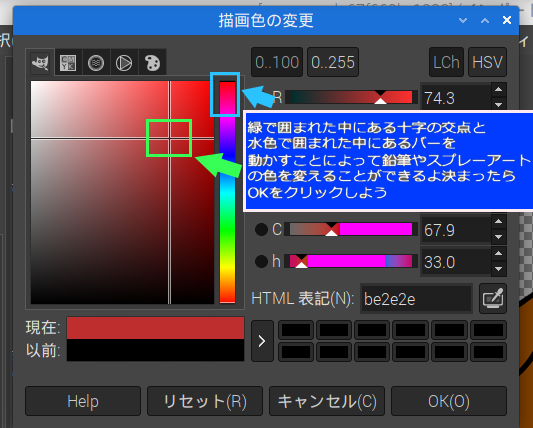
\includegraphics[width=8.654cm,height=4.325cm]{textbook-img126.png}\\
      4 色を変更しよう

      好きな色を選んでOKを\ruby{押}{お}します


      \bigskip
      \begin{minipage}{5.984cm}
        5
        今回は色を赤にしました。赤く囲んであるところの色が赤に変わっていることを確認してください。


      \end{minipage}
    \end{minipage}
  \end{minipage}

  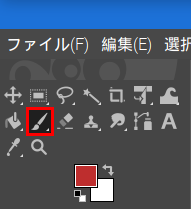
\includegraphics[width=1.866cm,height=4.15cm]{textbook-img127.png}
  \begin{minipage}[b]{6.663cm}
    6 次にお絵かきツールを選びます。

    赤色で囲われているところをクリックしてください。これで色付きの筆が使えるようになります。


    \bigskip

  \end{minipage}
\end{figure}
\clearpage
\begin{figure}[ht]
  \textbf{考え方(続き)}

  \begin{minipage}{\textwidth}
    \centering
    \begin{minipage}{5.76cm}
      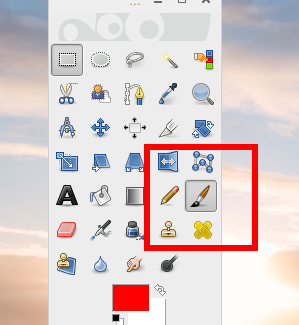
\includegraphics[width=5.05cm,height=4.796cm]{textbook-img130.png}\\
      7
      ツール\ruby{一覧}{いちらん}の下の文字が「ブラシで\ruby{描画}{びょうが}」に変わったことを確認しましょう。これで筆が使えるようになりました。
    \end{minipage}
    \hfill
    \begin{minipage}{10.2cm}
      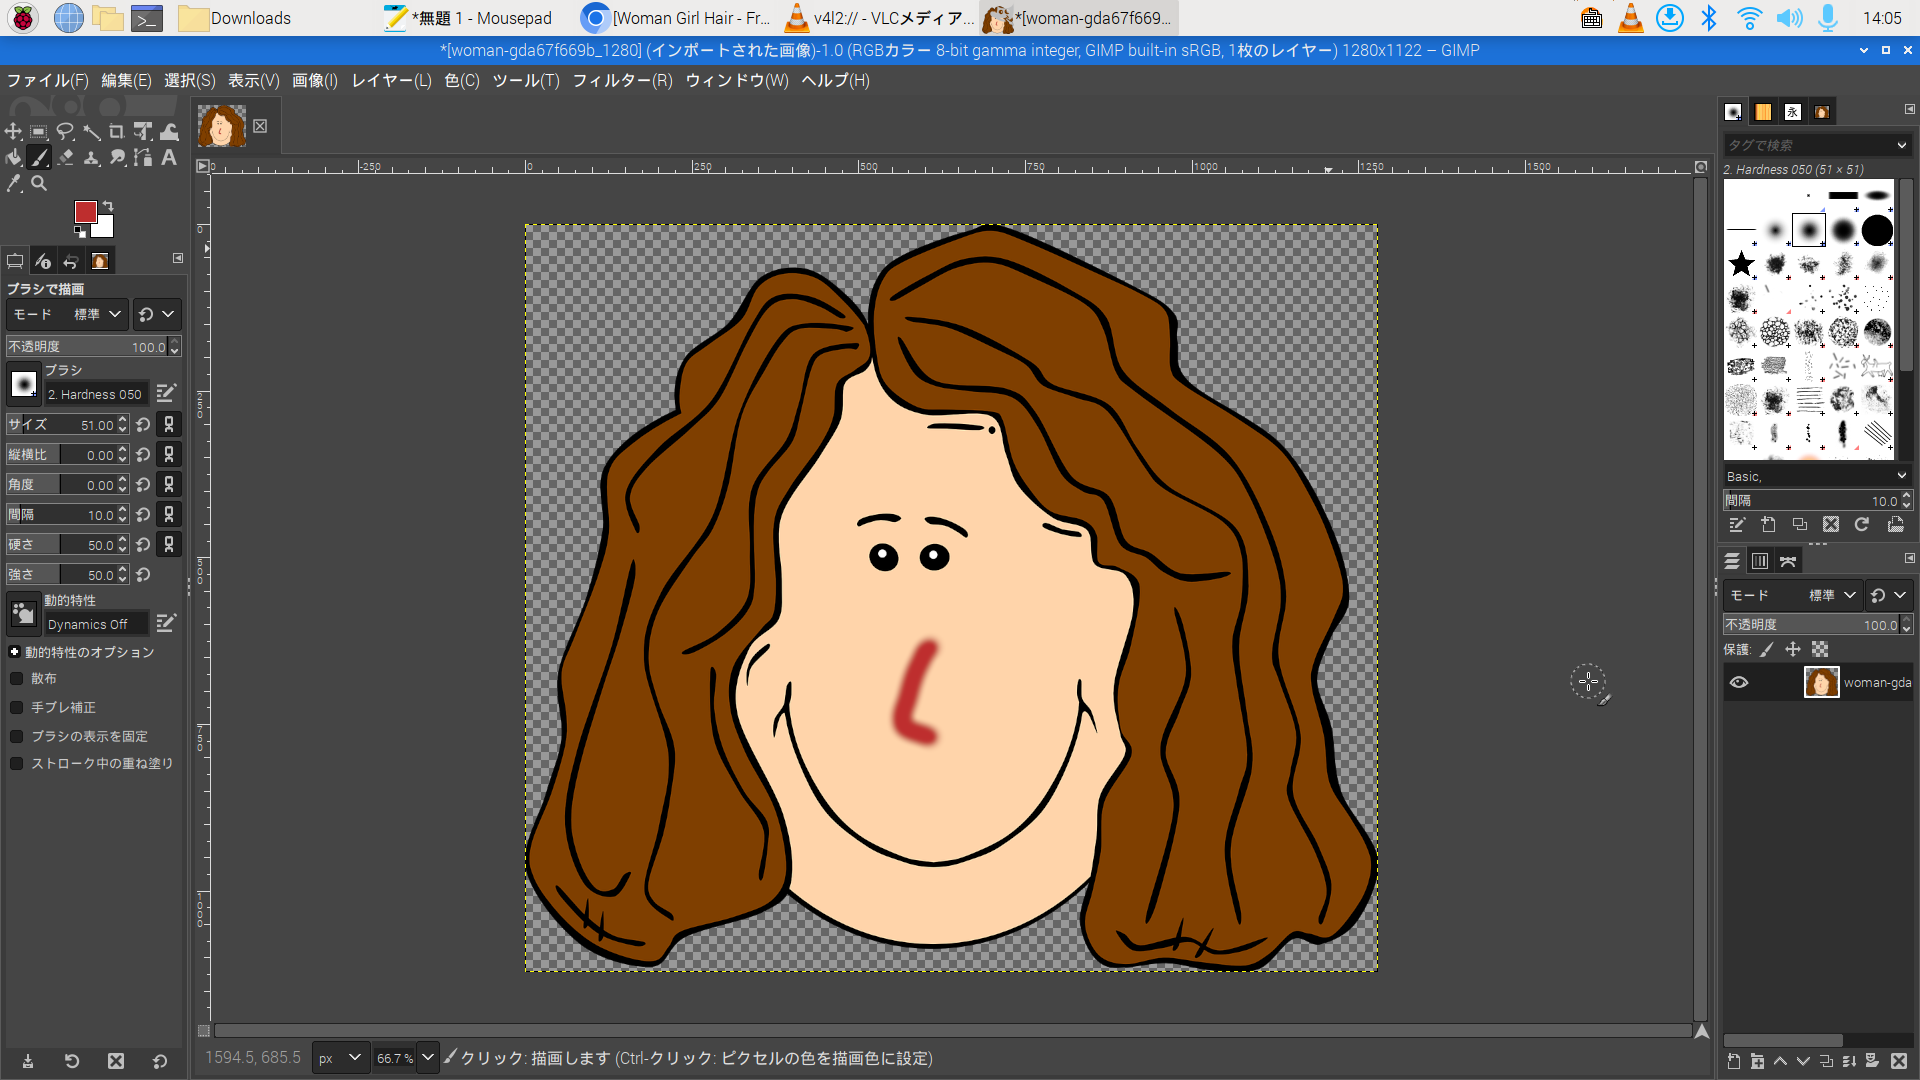
\includegraphics[width=10.134cm,height=5.697cm]{textbook-img131.png}\\
      8 左クリックをおしながら画像の上を\ruby{移動}{いどう}させると筆でお絵かきができます。いたずら書きをしてみてください
    \end{minipage}
  \end{minipage}


  \bigskip

  \begin{minipage}{\textwidth}
    \begin{minipage}{6.984cm}
      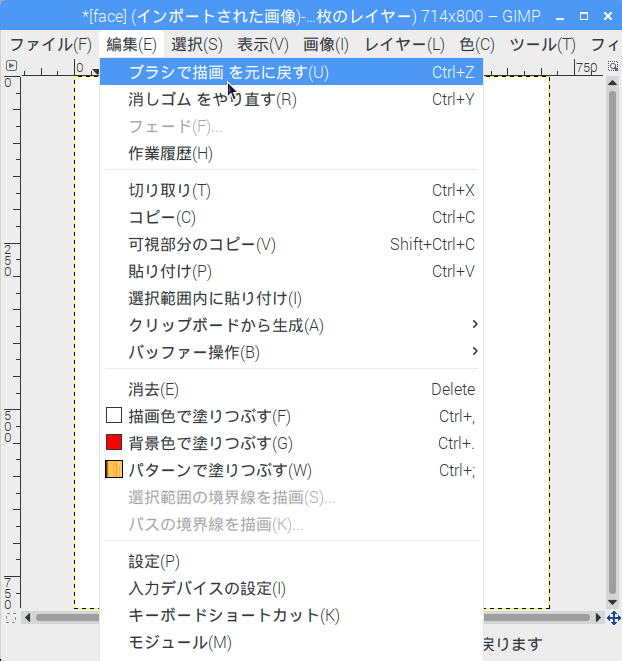
\includegraphics[width=6.228cm,height=6.618cm]{textbook-img132.png}\\
      9 \ruby{間違}{まちが}えてしまって、もとに戻したいとなったらメニューの編集からもとに\ruby{戻}{もど}すをクリックします。
    \end{minipage}
    \hfill
    \begin{minipage}{8.966cm}
      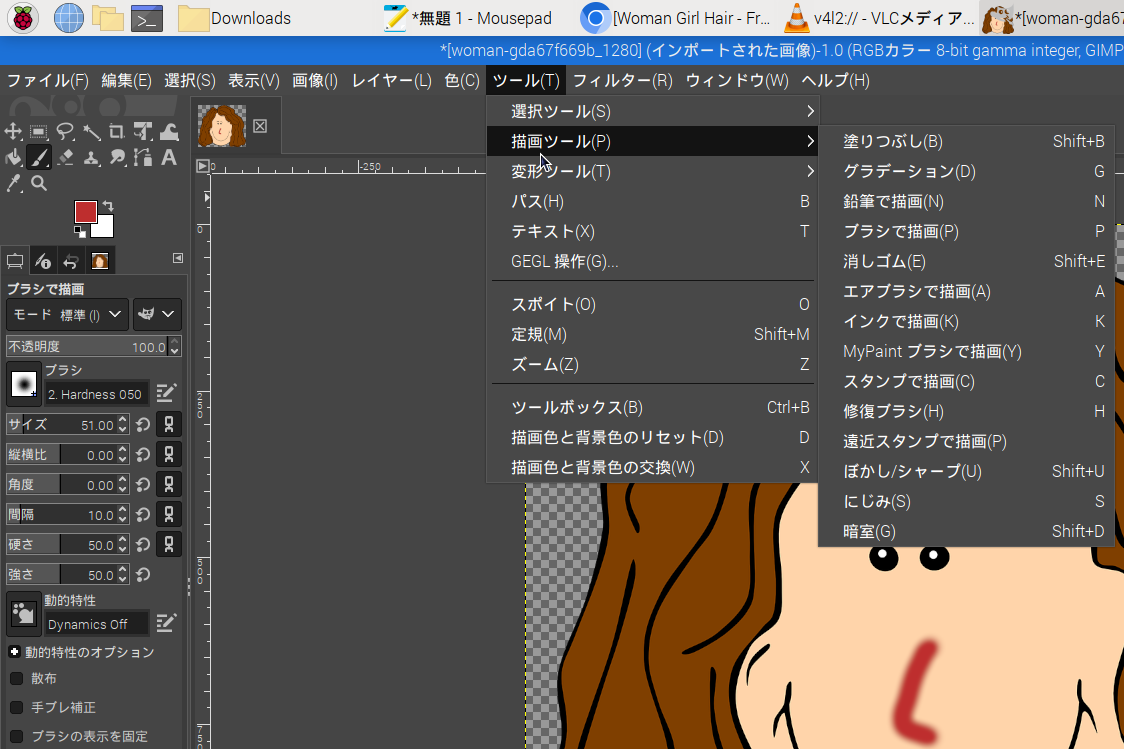
\includegraphics[width=8.881cm,height=4.997cm]{textbook-img133.png}\\
      10 他にもたくさんツールはあります。メニューのツール\ruby{欄}{らん}にある\ruby{描画}{びょうが}ツールで選べるよ。\ruby{鉛筆}{えんぴつ}、インクを試してみよう。書き方はいっしょで左クリックを押しながら移動だよ
    \end{minipage}
  \end{minipage}
\end{figure}

~

\vfill
\clearpage
\begin{figure}
  \textbf{考え方(続き)}


  編集しおわったら書き出しをします。

  \centering
  \begin{minipage}{13.237cm}
    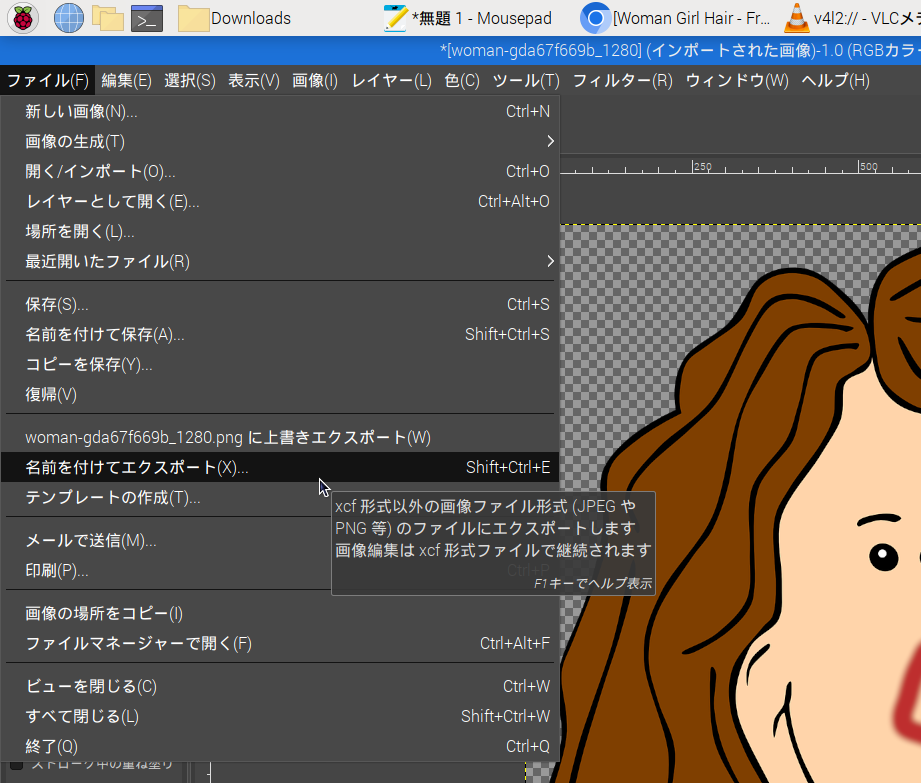
\includegraphics[width=13.178cm,height=7.408cm]{textbook-img138.png}\\
    11 編集がおわったら

    ファイルから名前を付けてエクスポートをクリック
  \end{minipage}

  \bigskip


  \begin{minipage}{\textwidth}
    \begin{minipage}{7.7cm}
      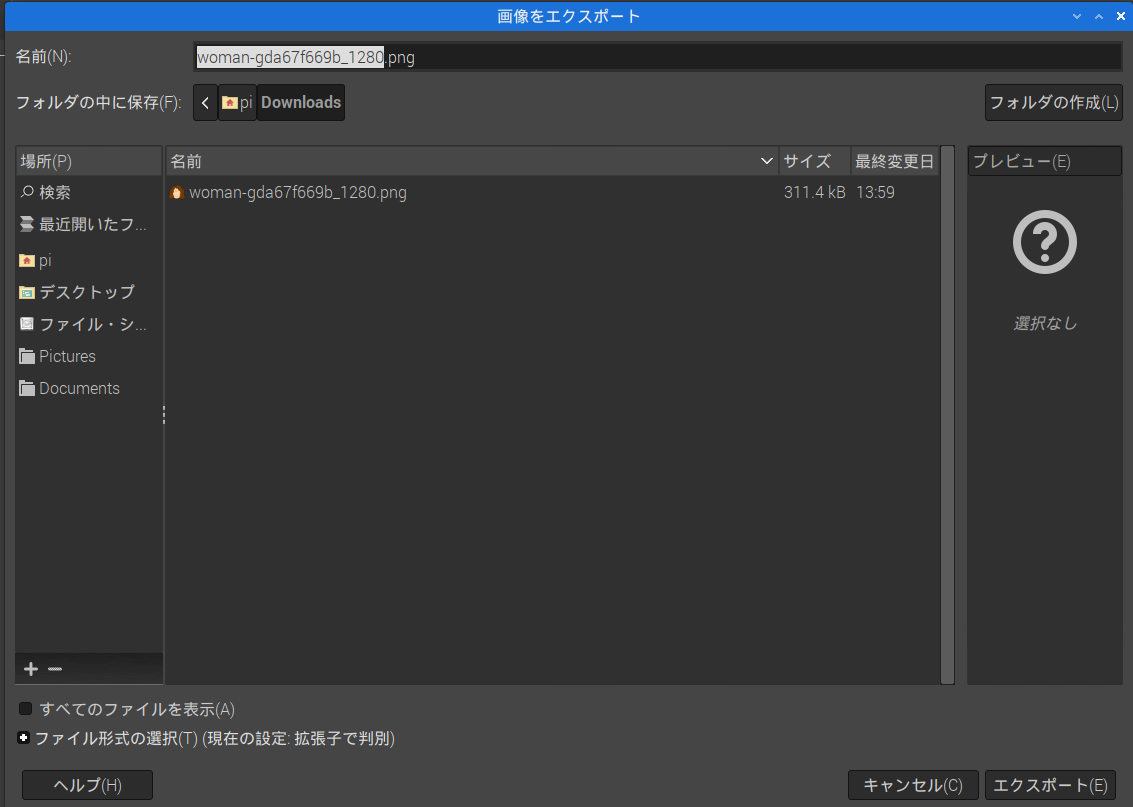
\includegraphics[width=7.615cm,height=5.209cm]{textbook-img137.png}\\
      12
      下のエクスポートをクリック(.jpegファイルから編集したならば12へ)
    \end{minipage}
    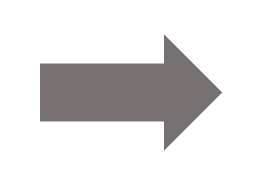
\includegraphics[width=1.919cm,height=1.365cm]{textbook-img135.png}
    \begin{minipage}{7.786cm}
      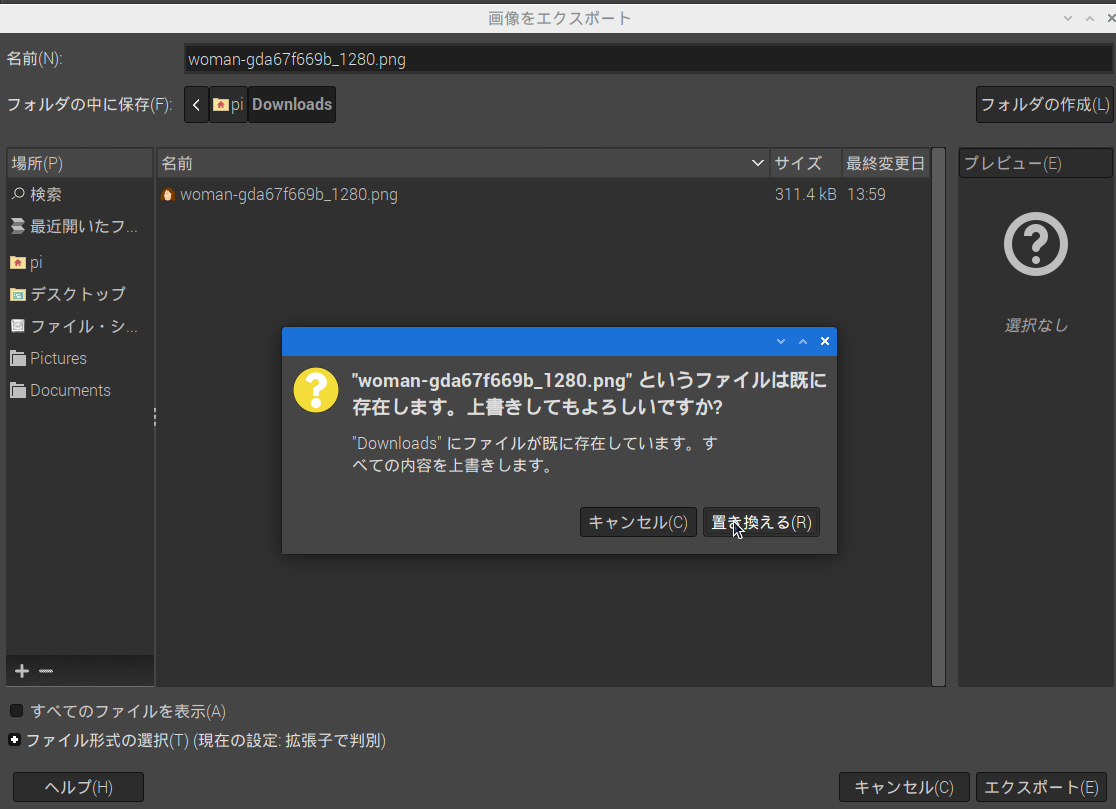
\includegraphics[width=7.352cm,height=5.756cm]{textbook-img136.png}\\
      13 置き換えるをクリック
    \end{minipage}
  \end{minipage}

  \bigskip


  \begin{minipage}{\textwidth}
    \begin{minipage}{8.074cm}
      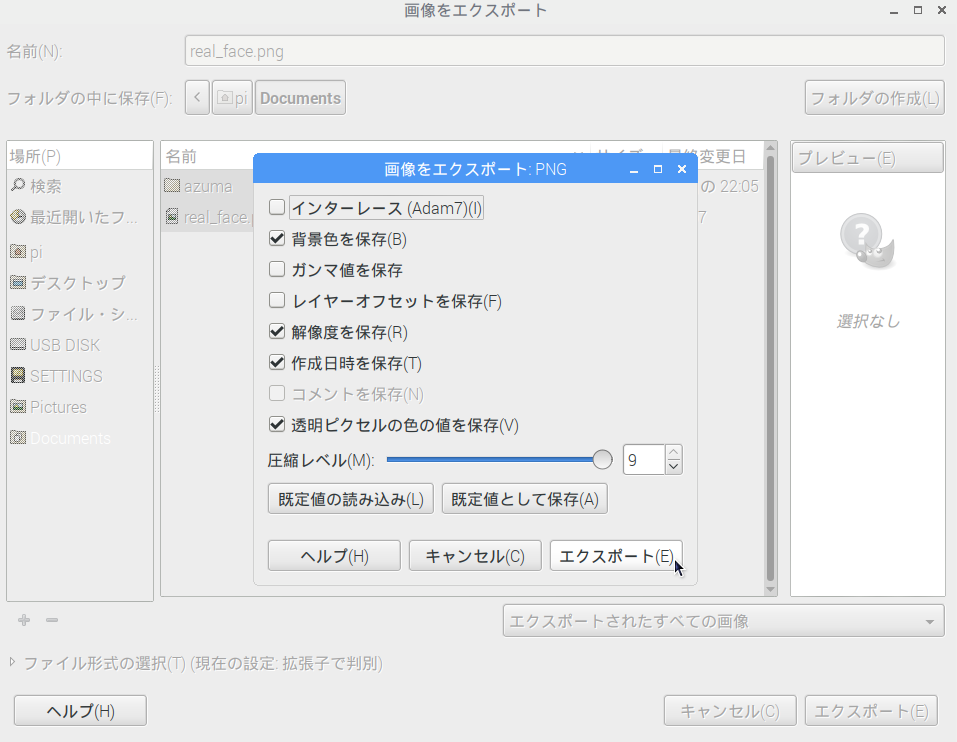
\includegraphics[width=7.721cm,height=5.26cm]{textbook-img134.png}\\
      14 エクスポートをクリック
    \end{minipage}
    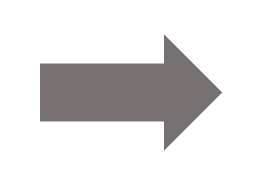
\includegraphics[width=1.919cm,height=1.365cm]{textbook-img135.png}
    \begin{minipage}{7.328cm}
      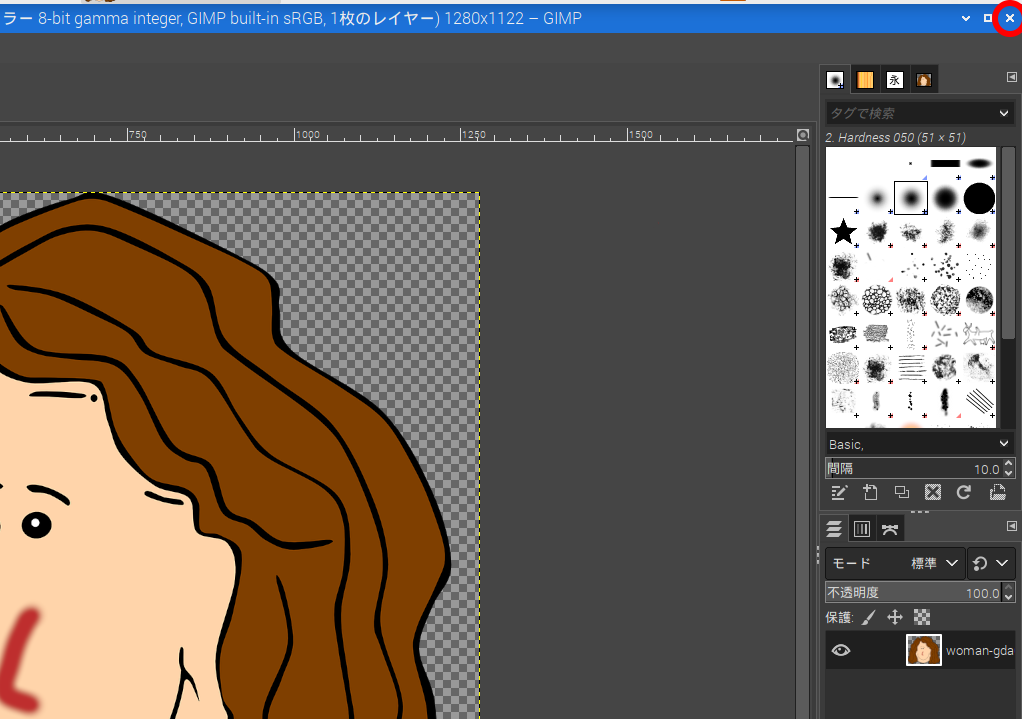
\includegraphics[width=7.061cm,height=5.653cm]{textbook-img1030.png}\\
      15
      右上の赤い丸で囲まれた×ボタンを押して、画像編集ツールを\ruby{閉}{と}じよう
    \end{minipage}
  \end{minipage}



\end{figure}
\clearpage

\begin{minipage}{0.45\linewidth}
  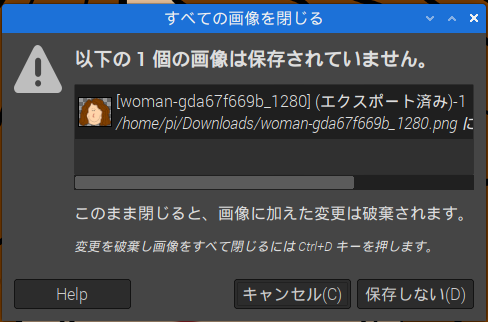
\includegraphics[width=\linewidth,height=5cm]{textbook-img1031.png}\\
  16 「保存されていません」というウィンドウがでます。これは、先ほど「エクスポート」したものとは別のことを言っていて、
  画像自体は保存されています。なので、気にせず「保存しない」をクリックしましょう
\end{minipage}
\hfill
\vspace{20pt}
\begin{minipage}{0.45\linewidth}
  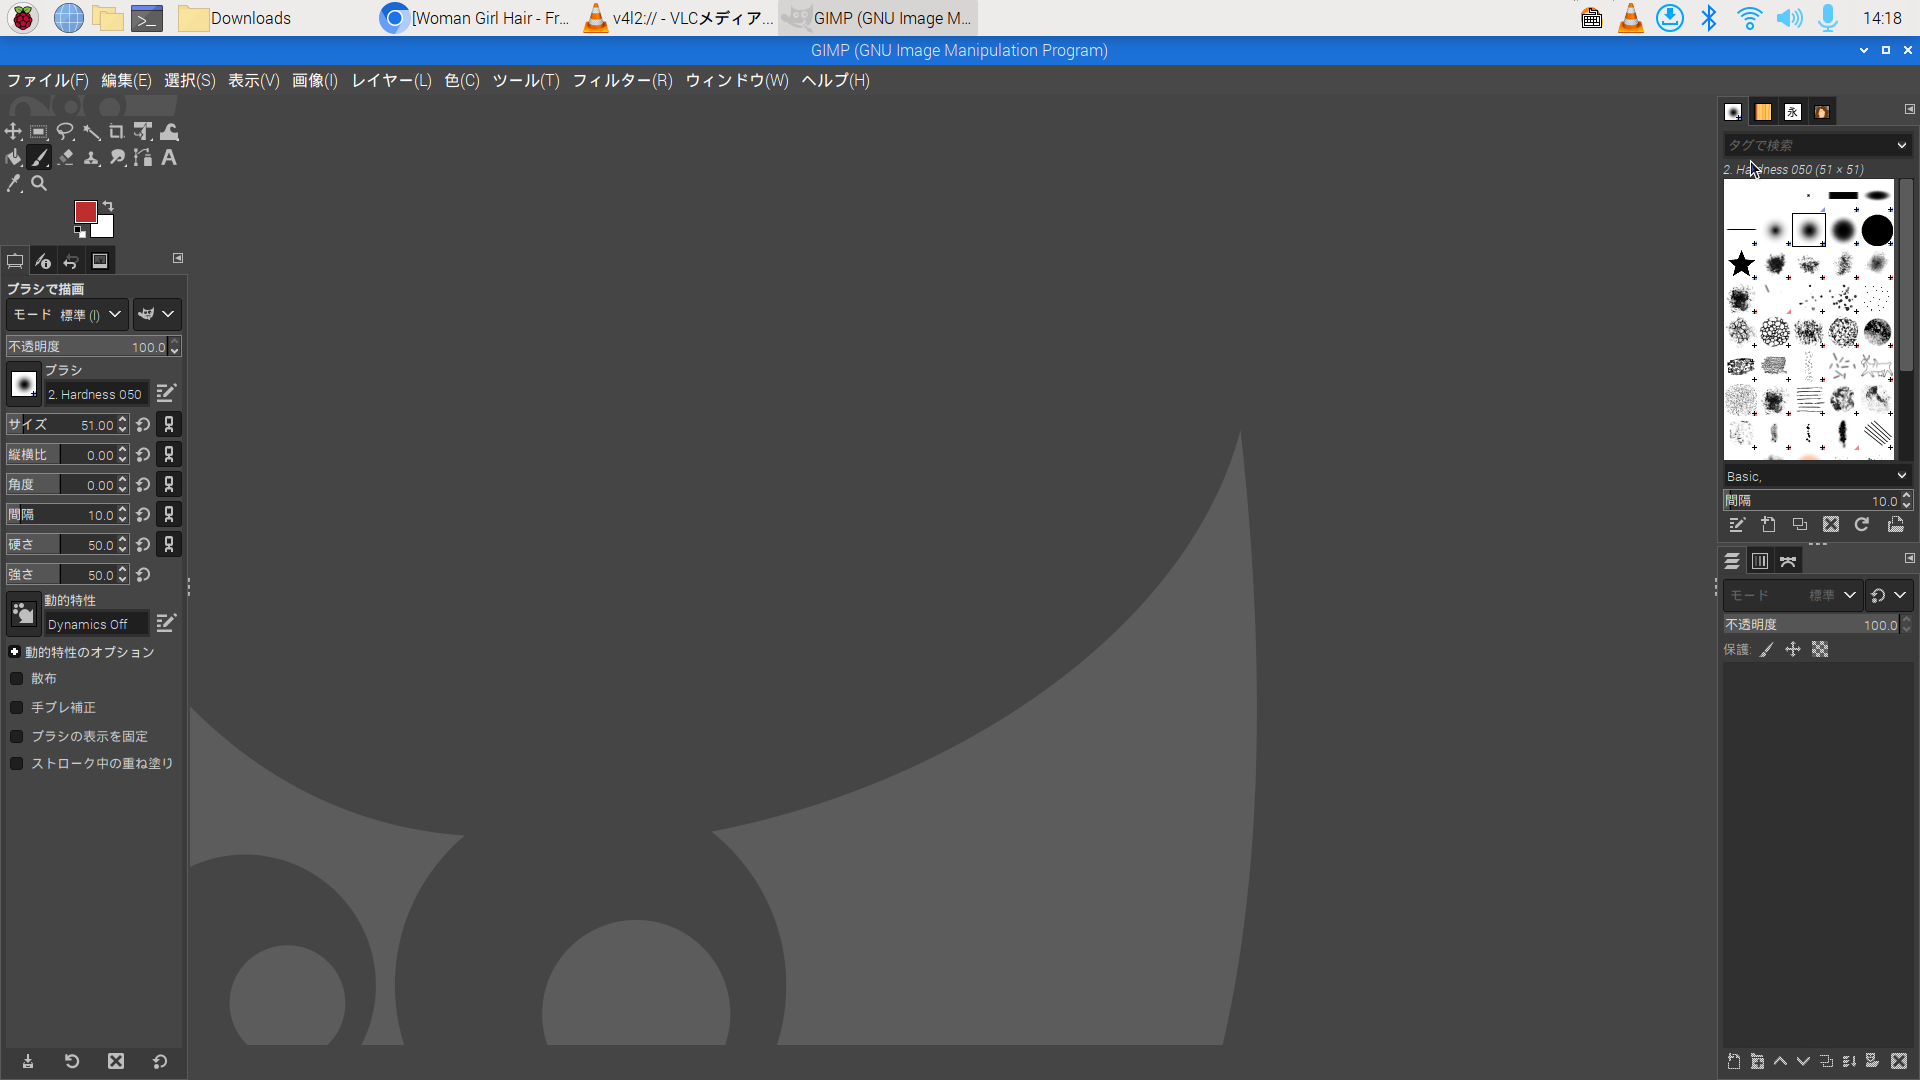
\includegraphics[width=\linewidth,height=5cm]{textbook-img1032.png}\\
  17 画像が消え、何もないウィンドウになります。右上の×ボタンをクリックして、画像編集ツールを閉じましょう
\end{minipage}
\begin{minipage}{0.45\linewidth}
  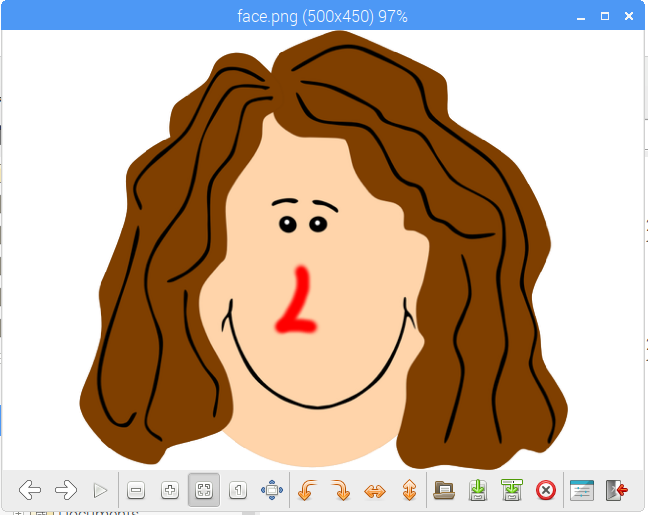
\includegraphics[width=\linewidth,height=5cm]{textbook-img139.png}\\
  18 画像ファイルを開いて確認してみよう
\end{minipage}
\hfill
\vspace{20pt}

\refstepcounter{Question}\theQuestion

”GIMP”を使って、自分の顔写真をさらに編集、加工してみよう

\begin{figure}[ht]
  \centering
  \begin{minipage}{9.082cm}
    {\upshape
      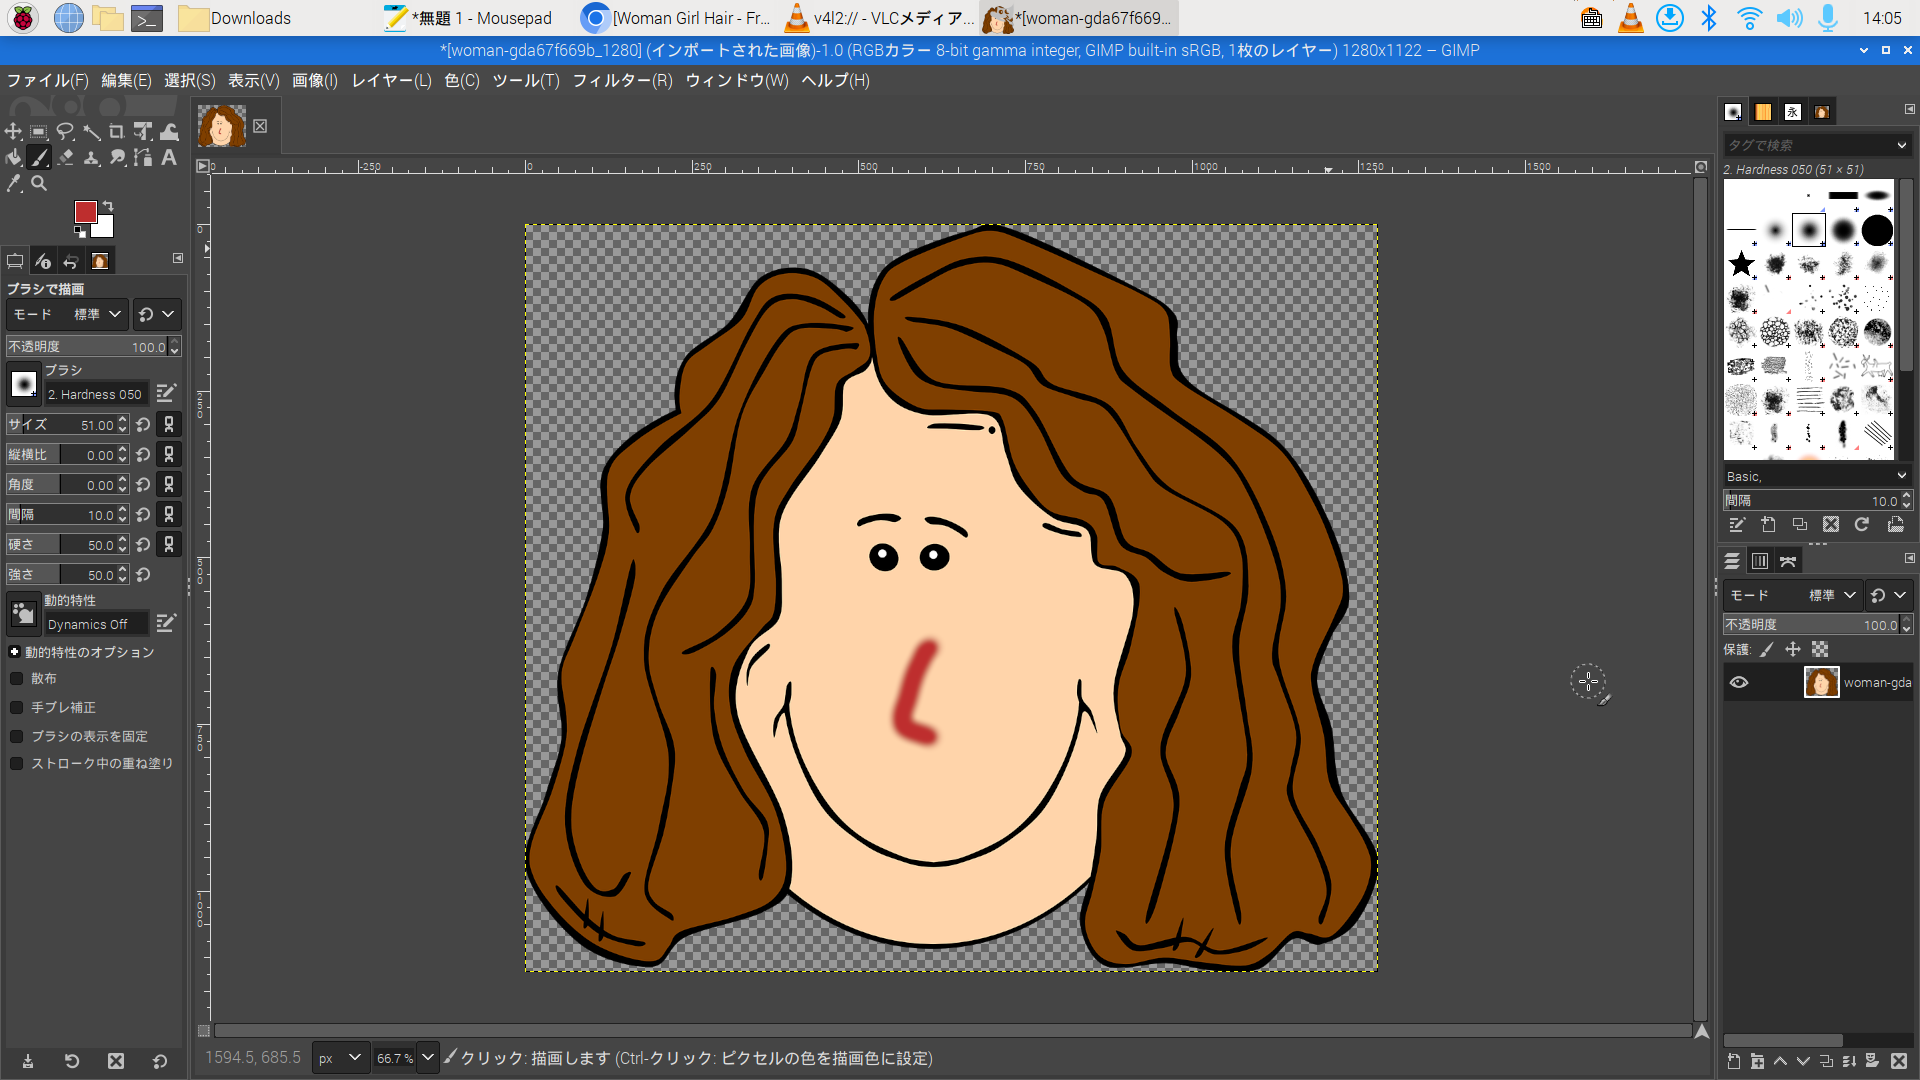
\includegraphics[width=9.082cm,height=5.105cm]{textbook-img131.png}
      \newline
      Figure \stepcounter{Figure}{\theFigure}: GIMP画像編集}
  \end{minipage}
\end{figure}

~
\vfill
\clearpage
\end{document}